Zine Sonia, CM\\
Mayafre Hadrien, TD\\
\chapter{Électrostatique}
\section{Loi de Coulomb, champ électrostatique}
\subsection{Loi de Coulomb}
La loi de Coulomb dicte les interactions entre des corps chargés ponctuels. La force qui s'applique sur des charges électrique dépend de leur signe. Soit $q_1$ et $q_2$ deux charges électriques ponctuelles : 
\begin{itemize}
    \item Si $q_1 q_2>0$ (charges de même signe) $\rightarrow$ force répulsive
    \item Si $q_1 q_2<0$ (charges de même signe) $\rightarrow$ force attractive
\end{itemize}

\begin{bclogo}[logo=\bccrayon,noborder=true,barre=snake]{Exemple}
\begin{minipage}{0.3\textwidth}
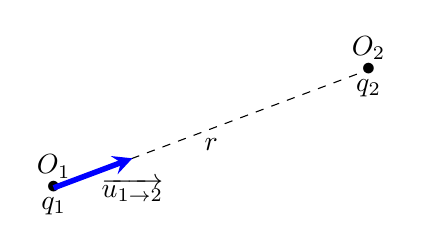
\begin{tikzpicture}[
scale=1,
axis/.style={very thick, ->, >=stealth'},
important line/.style={thick},
dashed line/.style={dashed, thin},
pile/.style={thick, ->, >=stealth', shorten <=2pt, shorten
>=2pt},
every node/.style={color=black}
]
\draw (4,1.5) node{$\bullet$} ;
\draw (4,1.5) node[above]{$O_2$} ;
\draw (4,1.5) node[below]{$q_2$} ;
\draw (0,0) node{$\bullet$} ;
\draw (0,0) node[above]{$O_1$} ;
\draw (0,0) node[below]{$q_1$} ;
\draw [dashed] (0,0) -- (4,1.5) ;
\draw (2,0.75) node[below]{$r$} ;
\draw[line width=2pt,blue,-stealth](0,0)--(1,0.375) node[below, yshift=-1mm]{$\boldsymbol{\overrightarrow{u_{1\rightarrow 2}}}$};
\end{tikzpicture}
\end{minipage}
\begin{minipage}{0.7\textwidth}
$r=||\overrightarrow{O_1 O_2}||$

$K=(4\pi \epsilon_0)^{-1}=9*10^9 Nm^2C^{-2}$ ; $\epsilon_0 = (36\pi*10^9)^{-1} Fm^{-1}$

\textbf{$\overrightarrow{f_{1\rightarrow2}}=K\dfrac{q_1 q_2}{r^2}\overrightarrow{u_{12}}$} : force exercée par $q_1$ sur $q_2$
\end{minipage}
\end{bclogo}

\chapter{Magnétisme et Électromgnétisme}
\include{PHY301/Ch52.tex}
\include{PHY301/Ch53.tex}
\chapter{Induction électromagnétique}

\begin{defi}
On appelle induction le phénomène qui conduit à l'apparition d'une force électromotrice engendrée par le magnétisme.
\end{defi}
\section{Force de Laplace}
\begin{defi}
La force de Laplace est la force électromagnétique qu'exerce un champ magnétique $\overrightarrow{B}$ sur un élément conducteur du circuit $\overrightarrow{dl}$ parcouru par une intensité $I$.
$$d\overrightarrow{F_{lap}}=I\overrightarrow{dl}\land\overrightarrow{B}$$
\end{defi}
\section{Loi de Faraday}
\begin{thm}[Loi de Faraday]
La variation temporelle du flux magnétique à travers un circuit fermé engendre une force électromotrice induite.
\begin{align*}
    & e=-\frac{d\phi}{dt} && \text{où}\ \phi=\iint\overrightarrow{B}\cdot\overrightarrow{d^2S}
\end{align*}
\end{thm}
\chapter{Équations de Maxwell}